% !TEX root = lectures.tex
\section{Oscillations}
\bigskip

\subsection{Harmonic Oscillator}

The harmonic oscillator is omnipresent in physics. Although students think of this as being related to springs, it, or an equivalent mathematical representation, appears in just about any problem where a mode is sitting near its potential energy minimum. At that point, $\partial_x V(x)=0$, and the first non-zero term (aside from a constant) in the potential energy is that of a harmonic oscillator. In a solid, sound modes (phonons) are built on a picture of coupled harmonic oscillators, and in relativistic field theory the fundamental interactions are also built on coupled oscillators positioned infinitesimally close to one another in space. The phenomena of a resonance of an oscillator driven at a fixed frequency plays out repeatedly in atomic, nuclear and high-energy physics, when quantum mechanically the evolution of a state oscillates according to $e^{-iEt}$ and exciting discrete quantum states has very similar mathematics as exciting discrete states of an oscillator.

The potential energy for a single particle as a function of its position $x$ can be written as a Taylor expansion about some point $x_0$
\begin{equation}
V(x)=V(x_0)+(x-x_0)\left.\partial_xV(x)\right|_{x_0}+\frac{1}{2}(x-x_0)^2\left.\partial_x^2V(x)\right|_{x_0}
+\frac{1}{3!}\left.\partial_x^3V(x)\right|_{x_0}+\cdots
\end{equation}
If the position $x_0$ is at the minimum of the resonance, the first two non-zero terms of the potential are
\begin{eqnarray}
V(x)&\approx& V(x_0)+\frac{1}{2}(x-x_0)^2\left.\partial_x^2V(x)\right|_{x_0},\\
\nonumber
&=&V(x_0)+\frac{1}{2}k(x-x_0)^2,~~~~k\equiv \left.\partial_x^2V(x)\right|_{x_0},\\
\nonumber
F&=&-\partial_xV(x)=-k(x-x_0).
\end{eqnarray}

Put into Newton's 2nd law (assuming $x_0=0$),
\begin{eqnarray}
m\ddot{x}&=&-kx,\\
x&=&A\cos(\omega_0 t-\phi),~~~\omega_0=\sqrt{k/m}.
\end{eqnarray}
Here $A$ and $\phi$ are arbitrary. Equivalently, one could have written this as $A\cos(\omega_0 t)+B\sin(\omega_0 t)$, or as the real part of $Ae^{i\omega_0 t}$. In this last case $A$ could be an arbitrary complex constant. Thus, there are 2 arbitrary constants (either $A$ and $B$ or $A$ and $\phi$, or the real and imaginary part of one complex constant. This is the expectation for a second order differential equation, and also agrees with the physical expectation that if you know a particle's initial velocity and position you should be able to define its future motion, and that those two arbitrary conditions should translate to two arbitrary constants.

A key feature of harmonic motion is that the system repeats itself after a time $T=1/f$, where $f$ is the frequency, and $\omega=2\pi f$ is the angular frequency. The period of the motion is independent of the amplitude. However, this independence is only exact when one can neglect higher terms of the potential, $x^3, x^4\cdots$. Once can neglect these terms for sufficiently small amplitudes, and for larger amplitudes the motion is no longer purely sinusoidal, and even though the motion repeats itself, the time for repeating the motion is no longer independent of the amplitude.

One can also calculate the velocity and the kinetic energy as a function of time,
\begin{eqnarray}
\dot{x}&=&-\omega_0A\sin(\omega_0 t-\phi),\\
\nonumber
T&=&\frac{1}{2}m\dot{x}^2=\frac{m\omega_0^2A^2}{2}\sin^2(\omega_0t-\phi),\\
\nonumber
&=&\frac{k}{2}A^2\sin^2(\omega_0t-\phi).
\end{eqnarray}
The total energy is then
\begin{equation}
E=T+U=\frac{1}{2}m\dot{x}^2+\frac{1}{2}kx^2=\frac{1}{2}kA^2.
\end{equation}
The total energy then goes as the square of the amplitude.

\example
A pendulum is an example of a harmonic oscillator. By expanding the kinetic and potential energies for small angles find the frequency for a pendulum of length $L$ with all the mass $m$ centered at the end by writing the eq.s of motion in the form of a harmonic oscillator.

{\bf Solution:} The potential energy and kinetic energies are (for $x$ being the displacement)
\begin{eqnarray*}
U&=&mgL(1-\cos\theta)\approx mgL\frac{x^2}{2L^2},\\
T&=&\frac{1}{2}mL^2\dot{\theta}^2\approx \frac{m}{2}\dot{x}^2.
\end{eqnarray*}
For small $x$ Newton's 2nd law becomes
\[
m\ddot{x}=-\frac{mg}{L}x,
\]
and the spring constant would appear to be $k=mg/L$, which makes the frequency equal to $\omega_0=\sqrt{g/L}$. Note that the frequency is independent of the mass.

\exampleend

\subsection{Damped Oscillators}

In this chapter we consider only the case where the damping force is proportional to the velocity. This is counter to dragging friction, where the force is proportional in strength to the normal force and independent of velocity, and is also inconsistent with wind resistance, where the magnitude of the drag force is proportional the square of the velocity. Rolling resistance does seem to be mainly proportional to the velocity. However, the main motivation for considering damping forces proportional to the velocity is that the math is more friendly. This is because the differential equation is linear, i.e. each term is of order $x$, $\dot{x}$, $\ddot{x}\cdots$, or even terms with no mention of $x$, and there are no terms such as $x^2$ or $x\ddot{x}$. The equations of motion for a spring with damping force $-b\dot{x}$ are
\begin{equation}
m\ddot{x}+b\dot{x}+kx=0.
\end{equation}
Just to make the solution a bit less messy, we rewrite this equation as
\begin{equation}
\label{eq:dampeddiffyq}
\ddot{x}+2\beta\dot{x}+\omega_0^2x=0,~~~~\beta\equiv b/2m,~\omega_0\equiv\sqrt{k/m}.
\end{equation}
Both $\beta$ and $\omega$ have dimensions of inverse time. To find solutions (see appendix C in the text) you must make an educated guess at the form of the solution. To do this, first realize that the solution will need an arbitrary normalization $A$ because the equation is linear. Secondly, realize that if the form is
\begin{equation}
x=Ae^{rt}
\end{equation}
that each derivative simply brings out an extra power of $r$. This means that the $Ae^{rt}$ factors out and one can simply solve for an equation for $r$. Plugging this form into Eq. (\ref{eq:dampeddiffyq}),
\begin{equation}
r^2+2\beta r+\omega_0^2=0.
\end{equation}
Because this is a quadratic equation there will be two solutions,
\begin{equation}
r=-\beta\pm\sqrt{\beta^2-\omega_0^2}.
\end{equation}
We refer to the two solutions as $r_1$ and $r_2$ corresponding to the $+$ and $-$ roots. As expected, there should be two arbitrary constants involved in the solution,
\begin{equation}
x=A_1e^{r_1t}+A_2e^{r_2t},
\end{equation}
where the coefficients $A_1$ and $A_2$ are determined by initial conditions.

The roots listed above, $\sqrt{\omega_0^2-\beta_0^2}$, will be imaginary if the damping  is small and $\beta<\omega_0$. In that case, $r$ is complex and the factor $e{rt}$ will have some oscillatory behavior. If the roots are real, there will only be exponentially decaying solutions. There are three cases:
\begin{enumerate}\itemsep 0pt
\item Underdamped: $\beta<\omega_0$
\begin{eqnarray}
x&=&A_1e^{-\beta t}e^{i\omega't}+A_2e^{-\beta t}e^{-i\omega't},~~\omega'\equiv\sqrt{\omega_0^2-\beta^2}\\
\nonumber
&=&(A_1+A_2)e^{-\beta t}\cos\omega't+i(A_1-A_2)e^{-\beta t}\sin\omega't.
\end{eqnarray}
Here we have made use of the identity $e^{i\omega't}=\cos\omega't+i\sin\omega't$. Because the constants are arbitrary, and because the real and imaginary parts are both solutions individually, we can simply consider the real part of the solution alone:
\begin{eqnarray}
\label{eq:homogsolution}
x&=&B_1e^{-\beta t}\cos\omega't+B_2e^{-\beta t}\sin\omega't,\\
\nonumber 
\omega'&\equiv&\sqrt{\omega_0^2-\beta^2}.
\end{eqnarray}

\item Critical dampling: $\beta=\omega_0$\\
In this case the two terms involving $r_1$ and $r_2$ are identical because $\omega'=0$. Because we need to arbitrary constants, there needs to be another solution. This is found by simply guessing, or by taking the limit of $\omega'\rightarrow 0$ from the underdamped solution. The solution is then
\begin{equation}
\label{eq:criticallydamped}
x=Ae^{-\beta t}+Bte^{-\beta t}.
\end{equation}
The critically damped solution is interesting because the solution approaches zero quickly, but does not oscillate. For a problem with zero initial velocity, the solution never crosses zero. This is a good choice for designing shock absorbers or swinging doors.
\item Overdamped: $\beta>\omega_0$
\begin{eqnarray}
x&=&A_1e^{-(\beta+\sqrt{\beta^2-\omega_0^2})t}+A_2e^{-(\beta-\sqrt{\beta^2-\omega_0^2})t}
\end{eqnarray}
This solution will also never pass the origin more than once, and then only if the initial velocity is strong and initially toward zero.
\end{enumerate}

\example
Given $b$, $m$ and $\omega_0$, find $x(t)$ for a particle whose initial position is $x=0$ and has initial velocity $v_0$ (assuming an underdamped solution).

{\bf Solution:} The solution is of the form,
\begin{eqnarray*}
x&=&e^{-\beta t}\left[A_1\cos(\omega' t)+A_2\sin\omega't\right],\\
\dot{x}&=&-\beta x+\omega'e^{-\beta t}\left[-A_1\sin\omega't+A_2\cos\omega't\right].\\
\omega'&\equiv&\sqrt{\omega_0^2-\beta^2},~~~\beta\equiv b/2m.
\end{eqnarray*}
From the initial conditions, $A_1=0$ because $x(0)=0$ and $\omega'A_2=v_0$. So 
\[
x=\frac{v_0}{\omega'}e^{-\beta t}\sin\omega't.
\]
\exampleend

\subsection{Sinusoidally Driven Oscillators}

Here, we consider the force
\begin{equation}
F=-kx-b\dot{x}+F_0\cos\omega t,
\end{equation}
which leads to the differential equation
\begin{equation}
\label{eq:drivenosc}
\ddot{x}+2\beta\dot{x}+\omega_0^2x=(F_0/m)\cos\omega t.
\end{equation}
Consider a single solution with no arbitrary constants, which we will call a {\it particular solution}, $x_p(t)$. It should be emphasized that this is {\bf A} particular solution, because there exists an infinite number of such solutions because the general solution should have two arbitrary constants. Now consider solutions to the same equation without the driving term, which include two arbitrary constants. These are called either {\it homogenous solutions} or {\it complementary solutions}, and were given in the previous section, e.g. Eq. (\ref{eq:homogsolution}) for the underdamped case. The homogenous solution already incorporates the two arbitrary constants, so any sum of a homogenous solution and a particular solution will represent the {\it general solution} of the equation. The general solution incorporates the two arbitrary constants $A$ and $B$ to accommodate the two initial conditions. One could have picked a different particular solution, i.e. the original particular solution plus any homogenous solution with the arbitrary constants $A_p$ and $B_p$ chosen at will. When one adds in the homogenous solution, which has adjustable constants with arbitrary constants $A'$ and $B'$, to the new particular solution, one can get the same general solution by simply adjusting the new constants such that $A'+A_p=A$ and $B'+B_p=B$. Thus, the choice of $A_p$ and $B_p$ are irrelevant, and when choosing the particular solution it is best to make the simplest choice possible.

To find a particular solution, one first guesses at the form,
\begin{equation}
\label{eq:partform}
x_p(t)=D\cos(\omega t-\delta),
\end{equation}
and rewrite the differential equation as
\begin{equation}
D\left\{-\omega^2\cos(\omega t-\delta)-2\beta\omega\sin(\omega t-\delta)+\omega_0^2\cos(\omega t-\delta)\right\}=\frac{F_0}{m}\cos(\omega t).
\end{equation}
One can now use angle addition formulas to get
\begin{eqnarray}
D\left\{(-\omega^2\cos\delta+2\beta\omega\sin\delta+\omega_0^2\cos\delta)\cos(\omega t)\right.\hspace*{36pt}&&\\
\nonumber
\left.+(-\omega^2\sin\delta-2\beta\omega\cos\delta+\omega_0^2\sin\delta)\sin(\omega t)\right\}
&=&\frac{F_0}{m}\cos(\omega t).
\end{eqnarray}
Both the $\cos$ and $\sin$ terms need to equate if the expression is to hold at all times. Thus, this becomes two equations
\begin{eqnarray}
D\left\{-\omega^2\cos\delta+2\beta\omega\sin\delta+\omega_0^2\cos\delta\right\}&=&\frac{F_0}{m}\\
\nonumber
-\omega^2\sin\delta-2\beta\omega\cos\delta+\omega_0^2\sin\delta&=&0.
\end{eqnarray}
After dividing by $\cos\delta$, the lower expression leads to
\begin{equation}
\tan\delta=\frac{2\beta\omega}{\omega_0^2-\omega^2}.
\end{equation}
Using the identities $\tan^2+1=\csc^2$ and $\sin^2+\cos\^2=1$, one can also express $\sin\delta$ and $\cos\delta$,
\begin{eqnarray}
\sin\delta&=&\frac{2\beta\omega}{\sqrt{(\omega_0^2-\omega^2)^2+4\omega^2\beta^2}},\\
\nonumber
\cos\delta&=&\frac{(\omega_0^2-\omega^2)}{\sqrt{(\omega_0^2-\omega^2)^2+4\omega^2\beta^2}}
\end{eqnarray}
Inserting the expressions for $\cos\delta$ and $\sin\delta$ into the expression for $D$,
\begin{equation}
\label{eq:Ddrive}
D=\frac{F_0/m}{\sqrt{(\omega_0^2-\omega^2)^2+4\omega^2\beta^2}}.
\end{equation}

For a given initial condition, e.g. initial displacement and velocity, one must add the homogenous solution then solve for the two arbitrary constants. However, because the homogenous solutions decay with time as $e^{-\beta t}$, the particular solution is all that remains at large times, and is therefore the steady state solution. Because the arbitrary constants are all in the homogenous solution, all memory of the initial conditions are lost at large times, $t>>1/\beta$.

The amplitude of the motion, $D$, is linearly proportional to the driving force ($F_0/m$), but also depends on the driving frequency $\omega$. For small $\beta$ the maximum will occur at $\omega=\omega_0$. This is referred to as a resonance. In the limit $\beta\rightarrow 0$ the amplitude at resonance approaches infinity. 

\subsection{Alternative Derivation for Driven Oscillators}

Here, we derive the same expressions as in Eq.s (\ref{eq:partform}-\ref{eq:Ddrive}) but express the driving forces as
\begin{eqnarray}
F(t)&=&F_0e^{i\omega t},
\end{eqnarray}
rather than as $F_0\cos\omega t$. The real part of $F$ is the same as before. For the differential equation,
\begin{eqnarray}
\label{eq:compdrive}
\ddot{x}+2\beta\dot{x}+\omega_0^2x&=&\frac{F_0}{m}e^{i\omega t},
\end{eqnarray}
one can treat $x(t)$ as an imaginary function. Because the operations $d^2/dt^2$ and $d/dt$ are real and thus do not mix the real and imaginary parts of $x(t)$, Eq. (\ref{eq:compdrive}) is effectively 2 equations. Because $e^{\omega t}=\cos\omega t+i\sin\omega t$, the real part of the solution for $x(t)$ gives the solution for a driving force $F_0\cos\omega t$, and the imaginary part of $x$ corresponds to the case where the driving force is $F_0\sin\omega t$. It is rather easy to solve for the complex $x$ in this case, and by taking the real part of the solution, one finds the answer for the $\cos\omega t$ driving force.

We assume a simple form for the particular solution
\begin{equation}
x_p=De^{i\omega t},
\end{equation}
where $D$ is a complex constant.

From Eq. (\ref{eq:compdrive}) one inserts the form for $x_p$ above to get
\begin{eqnarray}
D\left\{-\omega^2+2i\beta\omega+\omega_0^2\right\}e^{i\omega t}=(F_0/m)e^{i\omega t},\\
\nonumber
D=\frac{F_0/m}{(\omega_0^2-\omega^2)+2i\beta\omega}.
\end{eqnarray}
The norm and phase for $D=|D|e^{-i\delta}$ can be read by inspection,
\begin{equation}
|D|=\frac{F_0/m}{\sqrt{(\omega_0^2-\omega^2)^2+4\beta^2\omega^2}},~~~~\tan\delta=\frac{2\beta\omega}{\omega_0^2-\omega^2}.
\end{equation}
This is the same expression for $\delta$ as before. One then finds $x_p(t)$,
\begin{eqnarray}
\label{eq:fastdriven1}
x_p(t)&=&\Re\frac{(F_0/m)e^{i\omega t-i\delta}}{\sqrt{(\omega_0^2-\omega^2)^2+4\beta^2\omega^2}}\\
\nonumber
&=&\frac{(F_0/m)\cos(\omega t-\delta)}{\sqrt{(\omega_0^2-\omega^2)^2+4\beta^2\omega^2}}.
\end{eqnarray}
This is the same answer as before.
If one wished to solve for the case where $F(t)= F_0\sin\omega t$, the imaginary part of the solution would work
\begin{eqnarray}
\label{eq:fastdriven2}
x_p(t)&=&\Im\frac{(F_0/m)e^{i\omega t-i\delta}}{\sqrt{(\omega_0^2-\omega^2)^2+4\beta^2\omega^2}}\\
\nonumber
&=&\frac{(F_0/m)\sin(\omega t-\delta)}{\sqrt{(\omega_0^2-\omega^2)^2+4\beta^2\omega^2}}.
\end{eqnarray}

\example
Consider the damped and driven harmonic oscillator worked out above. Given $F_0, m,\beta$ and $\omega_0$, solve for the complete solution $x(t)$ for the case where $F=F_0\sin\omega t$ with initial conditions $x(t=0)=0$ and $v(t=0)=0$. Assume the underdamped case.

{\bf Solution:}
The general solution including the arbitrary constants includes both the homogenous and particular solutions,
\begin{eqnarray*}
x(t)&=&\frac{F_0}{m}\frac{\sin(\omega t-\delta)}{\sqrt{(\omega_0^2-\omega^2)^2+4\beta^2\omega^2}}
+A\cos\omega't e^{-\beta t}+B\sin\omega't e^{-\beta t}.
\end{eqnarray*}
The quantities $\delta$ and $\omega'$ are given earlier in the section, $\omega'=\sqrt{\omega_0^2-\beta^2}, \delta=\tan^{-1}(2\beta\omega/(\omega_0^2-\omega^2)$. Here, solving the problem means finding the arbitrary constants $A$ and $B$. Satisfying the initial conditions for the initial position and velocity:
\begin{eqnarray*}
x(t=0)=0&=&-\eta\sin\delta+A,\\
v(t=0)=0&=&\omega\eta\cos\delta-\beta A+\omega'B,\\
\eta&\equiv&\frac{F_0}{m}\frac{1}{\sqrt{(\omega_0^2-\omega^2)^2+4\beta^2\omega^2}}.
\end{eqnarray*}
The problem is now reduced to 2 equations and 2 unknowns, $A$ and $B$. The solution is
\begin{eqnarray}
A&=& \eta\sin\delta ,~~~B=\frac{-\omega\eta\cos\delta+\beta\eta\sin\delta}{\omega'}.
\end{eqnarray}

\exampleend

\subsection{Resonance Widths; the $Q$ factor}

From the previous two sections, the particular solution for a driving force, $F=F_0\cos\omega t$, is
\begin{eqnarray}
x_p(t)&=&\frac{F_0/m}{\sqrt{(\omega_0^2-\omega^2)^2+4\omega^2\beta^2}}\cos(\omega_t-\delta),\\
\nonumber
\delta&=&\tan^{-1}\left(\frac{2\beta\omega}{\omega_0^2-\omega^2}\right).
\end{eqnarray}
If one fixes the driving frequency $\omega$ and adjusts the fundamental frequency $\omega_0=\sqrt{k/m}$, the maximum amplitude occurs when $\omega_0=\omega$ because that is when the term from the denominator $(\omega_0^2-\omega^2)^2+4\omega^2\beta^2$ is at a minimum. This is akin to dialing into a radio station. However, if one fixes $\omega_0$ and adjusts the driving frequency one minimize with respect to $\omega$, e.g. set 
\begin{equation}
\frac{d}{d\omega}\left[(\omega_0^2-\omega^2)^2+4\omega^2\beta^2\right]=0,
\end{equation}
and one finds that the maximum amplitude occurs when $\omega=\sqrt{\omega_0^2-2\beta^2}$. If $\beta$ is small relative to $\omega_0$, one can simply state that the maximum amplitude is
\begin{equation}
x_{\rm max}\approx\frac{F_0}{2m\beta \omega_0}.
\end{equation}
\begin{figure}
\centerline{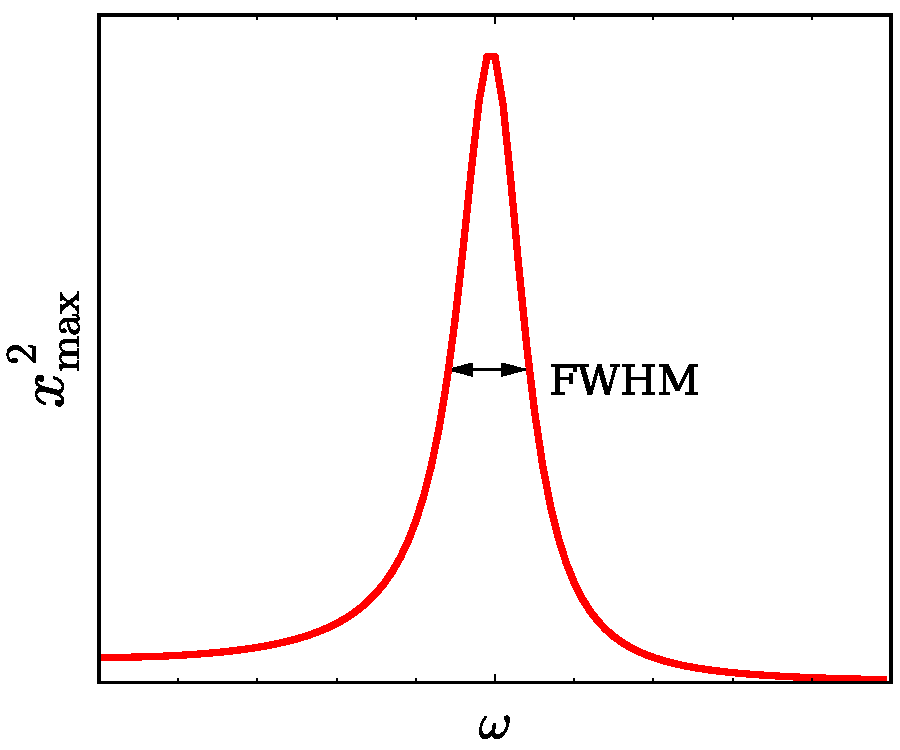
\includegraphics[width=0.32\textwidth]{figs/qfactor}}
\caption{\label{fig:qfactor}
The maximum amplitude squared of the steady-state motion of a sinusoidally driven harmonic oscillator is shown as a function of the driving frequency $\omega$. This peaks near the fundamental frequency $\omega_0$ and the full-width-half-maximum, $FWHM$, is given by the damping, $2\beta$.}
\end{figure}
Figure \ref{fig:qfactor} displays the maximum amplitude squared as a function of $\omega$, and  one can see the peak at $\omega\approx\omega_0$. The squared amplitude is usually more the quantity of interest than the amplitude because the power being absorbed by the oscillator is proportional to the square of the amplitude, not the amplitude. The width of the peak is quantified by the full-width-half-maximum, sometimes called $FWHM$ and can be found by finding the frequency difference, $\omega-\omega_0$, such that the maximum response falls by a factor of two,
\begin{eqnarray}
\frac{4\omega^2\beta^2}{(\omega_0^2-\omega^2)^2+4\omega^2\beta^2}=\frac{1}{2}.
\end{eqnarray}
For small damping this occurs when $\omega=\omega_0\pm \beta$, so the $FWHM\approx 2\beta$. For the purposes of tuning to a specific frequency, one wants the width to be as small as possible. The ratio of $\omega_0$ to $FWHM$ is known as the {\it quality} factor, or $Q$ factor,
\begin{equation}
Q\equiv \frac{\omega_0}{2\beta}.
\end{equation}

\subsection{Principal of Superposition and Periodic Forces (Fourier Transforms)}

If one has several driving forces, $F(t)=\sum_n F_n(t)$, one can find the particular solution to each $F_n$, $x_{pn}(t)$, and the particular solution for the entire driving force is 
\begin{equation}
x_p(t)=\sum_nx_{pn}(t).
\end{equation}
This is known as the principal of superposition. It only applies when the homogenous equation is linear. If there were an anharmonic term such as $x^3$ in the homogenous equation, then when one summed various solutions, $x=(\sum_n x_n)^2$, one would get cross terms. Superposition is especially useful when $F(t)$ can be written as a sum of sinusoidal terms, because the solutions for each sinusoidal term is analytic, and are given in the previous two subsections. 

Driving forces are often periodic, even when they are not sinusoidal. Periodicity implies that for some time $\tau$
\begin{eqnarray}
F(t+\tau)=F(t). 
\end{eqnarray}
One example of a non-sinusoidal periodic force is a square wave. Many components in electric circuits are non-linear, e.g. diodes, which makes many wave forms non-sinusoidal even when the circuits are being driven by purely sinusoidal sources.

For the sinusoidal example studied in the previous subsections the period is $\tau=2\pi/\omega$. However, higher harmonics can also satisfy the periodicity requirement. In general, any force that satisfies the periodicity requirement can be expressed as a sum over harmonics,
\begin{equation}
F(t)=\frac{f_0}{2}+\sum_{n>0} f_n\cos(2n\pi t/\tau)+g_n\sin(2n\pi t/\tau).
\end{equation}
From the previous subsection, one can write down the answer for $x_{pn}(t)$, by substituting $f_n/m$ or $g_n/m$ for $F_0/m$ into Eq.s (\ref{eq:fastdriven1}) or (\ref{eq:fastdriven2}) respectively. By writing each factor $2n\pi t/\tau$ as $n\omega t$, with $\omega\equiv 2\pi/\tau$,
\begin{equation}
\label{eq:fourierdef1}
F(t)=\frac{f_0}{2}+\sum_{n>0}f_n\cos(n\omega t)+g_n\sin(n\omega t).
\end{equation}
The solutions for $x(t)$ then come from replacing $\omega$ with $n\omega$ for each term in the particular solution in Eq.s (\ref{eq:partform}-\ref{eq:Ddrive}),
\begin{eqnarray}
x_p(t)&=&\frac{f_0}{2k}+\sum_{n>0} \alpha_n\cos(n\omega t-\delta_n)+\beta_n\sin(n\omega t-\delta_n),\\
\nonumber
\alpha_n&=&\frac{f_n/m}{\sqrt{((n\omega)^2-\omega_0^2)+4\beta^2n^2\omega^2}},\\
\nonumber
\beta_n&=&\frac{g_n/m}{\sqrt{((n\omega)^2-\omega_0^2)+4\beta^2n^2\omega^2}},\\
\nonumber
\delta_n&=&\tan^{-1}\left(\frac{2\beta n\omega}{\omega_0^2-n^2\omega^2}\right).
\end{eqnarray}
Because the forces have been applied for a long time, any non-zero damping eliminates the homogenous parts of the solution, so one need only consider the particular solution for each $n$.

The problem will considered solved if one can find expressions for the coefficients $f_n$ and $g_n$, even though the solutions are expressed as an infinite sum. The coefficients can be extracted from the function $F(t)$ by
\begin{eqnarray}
\label{eq:fourierdef2}
f_n&=&\frac{2}{\tau}\int_{-\tau/2}^{\tau/2} dt~F(t)\cos(2n\pi t/\tau),\\
\nonumber
g_n&=&\frac{2}{\tau}\int_{-\tau/2}^{\tau/2} dt~F(t)\sin(2n\pi t/\tau).
\end{eqnarray}

To check the consistency of these expressions and to verify Eq. (\ref{eq:fourierdef2}), one can insert the expansion of $F(t)$ in Eq. (\ref{eq:fourierdef1}) into the expression for the coefficients in Eq. (\ref{eq:fourierdef2}) and see whether
\begin{eqnarray}
f_n&=?&\frac{2}{\tau}\int_{-\tau/2}^{\tau/2} dt~\left\{
\frac{f_0}{2}+\sum_{m>0}f_m\cos(m\omega t)+g_m\sin(m\omega t)
\right\}\cos(n\omega t).
\end{eqnarray}
Immediately, one can throw away all the terms with $g_m$ because they convolute an even and an odd function. The term with $f_0/2$ disappears because $\cos(n\omega t)$ is equally positive and negative over the interval and will integrate to zero. For all the terms $f_m\cos(m\omega t)$ appearing in the sum, one can use angle addition formulas to see that $\cos(m\omega t)\cos(n\omega t)=(1/2)(\cos[(m+n)\omega t]+\cos[(m-n)\omega t]$. This will integrate to zero unless $m=n$. In that case the $m=n$ term gives
\begin{equation}
\int_{-\tau/2}^{\tau/2}dt~\cos^2(m\omega t)=\frac{\tau}{2},
\end{equation}
and
\begin{eqnarray}
f_n&=?&\frac{2}{\tau}\int_{-\tau/2}^{\tau/2} dt~f_n/2\\
\nonumber
&=&f_n~\checkmark.
\end{eqnarray}
The same method can be used to check for the consistency of $g_n$.

\example
Consider the driving force:
\begin{equation}
F(t)=At/\tau,~~-\tau/2<t<\tau/2,~~~F(t+\tau)=F(t).
\end{equation}
Find the Fourier coefficients $f_n$ and $g_n$ for all $n$ using Eq. (\ref{eq:fourierdef2}).

{\bf Solution:} Only the odd coefficients enter by symmetry, i.e. $f_n=0$. One can find $g_n$ integrating by parts,
\begin{eqnarray}
\label{eq:fouriersolution}
g_n&=&\frac{2}{\tau}\int_{-\tau/2}^{\tau/2}dt~\sin(n\omega t) \frac{At}{\tau}\\
\nonumber
u&=&t,~dv=\sin(n\omega t)dt,~v=-\cos(n\omega t)/(n\omega),\\
\nonumber
g_n&=&\frac{-2A}{n\omega \tau^2}\int_{-\tau/2}^{\tau/2}dt~\cos(n\omega t)
+\left.2A\frac{-t\cos(n\omega t)}{n\omega\tau^2}\right|_{-\tau/2}^{\tau/2}.
\end{eqnarray}
The first term is zero because $\cos(n\omega t)$ will be equally positive and negative over the interval. Using the fact that $\omega\tau=2\pi$,
\begin{eqnarray}
g_n&=&-\frac{2A}{2n\pi}\cos(n\omega\tau/2)\\
\nonumber
&=&-\frac{A}{n\pi}\cos(n\pi)\\
\nonumber
&=&\frac{A}{n\pi}(-1)^{n+1}.
\end{eqnarray}
The true function is compared to the expansion in Fig. \ref{fig:triangle} where the sum is cut off at finite $n$.
\begin{figure}
\centerline{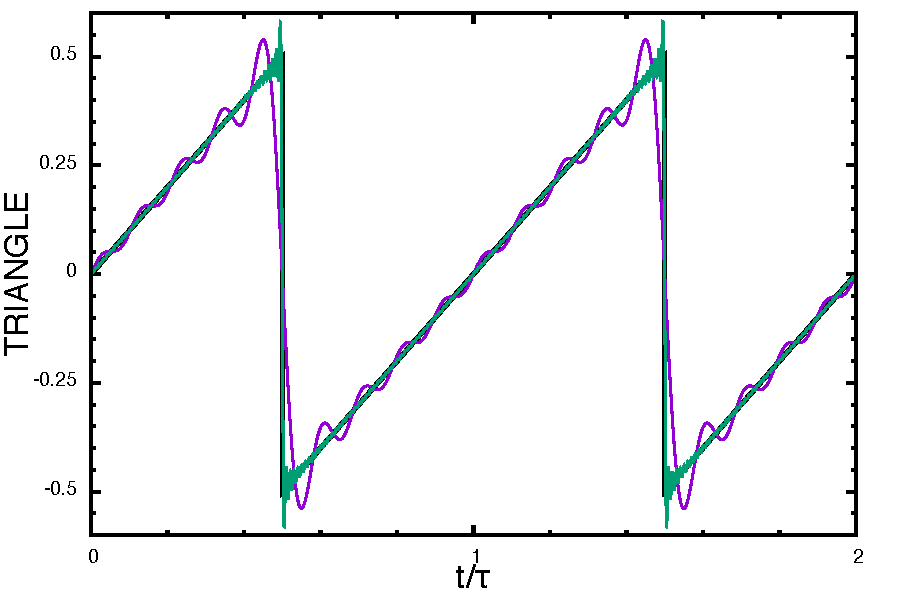
\includegraphics[width=0.6\textwidth]{figs/triangle}}
\caption{\label{fig:triangle}
The periodic function $F(t)=t/\tau, |t|<\tau/2$ (black) is compared to the Fourier expansion described in Eq. (\ref{eq:fouriersolution}) with 10 terms (red) or 100 terms (green).}
\end{figure}

\exampleend

\subsection{Response to Transient Force}

Consider a particle at rest in the bottom of an underdamped harmonic oscillator, that then feels a sudden impulse, or change in momentum, $I=F\Delta t$ at $t=0$. This increases the velocity immediately by an amount $v_0=I/m$ while not changing the position. One can then solve the trajectory by solving Eq. (\ref{eq:homogsolution}) with initial conditions $v_0=I/m$ and $x_0=0$. This gives
\begin{equation}
x(t)=\frac{I}{m\omega'}e^{-\beta t}\sin\omega't, ~~t>0.
\end{equation}
Here, $\omega'=\sqrt{\omega_0^2-\beta^2}$. For an impulse $I_i$ that occurs at time $t_i$ the trajectory would be
\begin{equation}
x(t)=\frac{I_i}{m\omega'}e^{-\beta (t-t_i)}\sin[\omega'(t-t_i)] \Theta(t-t_i),
\end{equation}
where $\Theta(t-t_i)$ is a step function, i.e. $\Theta(x)$ is zero for $x<0$ and unity for $x>0$. If there were several impulses linear superposition tells us that we can sum over each contribution,
\begin{equation}
x(t)=\sum_i\frac{I_i}{m\omega'}e^{-\beta(t-t_i)}\sin[\omega'(t-t_i)]\Theta(t-t_i)
\end{equation} 

Now one can consider a series of impulses at times separated by $\Delta t$, where each impulse is given by $F_i\Delta t$. The sum above now becomes an integral,
\begin{eqnarray}\label{eq:Greeny}
x(t)&=&\int_{-\infty}^\infty dt'~F(t')\frac{e^{-\beta(t-t')}\sin[\omega'(t-t')]}{m\omega'}\Theta(t-t')\\
\nonumber
&=&\int_{-\infty}^\infty dt'~F(t')G(t-t'),\\
\nonumber
G(\Delta t)&=&\frac{e^{-\beta\Delta t}\sin[\omega' \Delta t]}{m\omega'}\Theta(\Delta t)
\end{eqnarray}
The quantity $e^{-\beta(t-t')}\sin[\omega'(t-t')]/m\omega'\Theta(t-t')$ is called a Green's function, $G(t-t')$. It describes the response at $t$ due to a force applied at a time $t'$, and is a function of $t-t'$. The step function ensures that the response does not occur before the force is applied. One should remember that the form for $G$ would change if the oscillator were either critically- or over-damped.

When performing the integral in Eq. (\ref{eq:Greeny}) one can use angle addition formulas to factor out the part with the $t'$ dependence in the integrand,
\begin{eqnarray}
\label{eq:Greeny2}
x(t)&=&\frac{1}{m\omega'}e^{-\beta t}\left[I_c(t)\sin(\omega't)-I_s(t)\cos(\omega't)\right],\\
\nonumber
I_c(t)&\equiv&\int_{-\infty}^t dt'~F(t')e^{\beta t'}\cos(\omega't'),\\
\nonumber
I_s(t)&\equiv&\int_{-\infty}^t dt'~F(t')e^{\beta t'}\sin(\omega't').
\end{eqnarray}
If the time $t$ is beyond any time at which the force acts, $F(t'>t)=0$, the coefficients $I_c$ and $I_s$ become independent of $t$. 

\example
Consider an undamped oscillator ($\beta\rightarrow 0$), with characteristic frequency $\omega_0$ and mass $m$, that is at rest until it feels a force described by a Gaussian form,
\begin{eqnarray*}
F(t)&=&F_0 \exp\left\{\frac{-t^2}{2\tau^2}\right\}.
\end{eqnarray*}
For large times ($t>>\tau$), where the force has died off, find $x(t)$.\\
{\bf Solution:} Solve for the coefficients $I_c$ and $I_s$ in Eq. (\ref{eq:Greeny2}). Because the Gaussian is an even function, $I_s=0$, and one need only solve for $I_c$,
\begin{eqnarray*}
I_c&=&F_0\int_{-\infty}^\infty dt'~e^{-t^{\prime 2}/(2\tau^2)}\cos(\omega_0 t')\\
&=&\Re F_0 \int_{-\infty}^\infty dt'~e^{-t^{\prime 2}/(2\tau^2)}e^{i\omega_0 t'}\\
&=&\Re F_0 \int_{-\infty}^\infty dt'~e^{-(t'-i\omega_0\tau^2)^2/(2\tau^2)}e^{-\omega_0^2\tau^2/2}\\
&=&F_0\tau \sqrt{2\pi} e^{-\omega_0^2\tau^2/2}.
\end{eqnarray*}
The third step involved completing the square, and the final step used the fact that the integral
\begin{eqnarray*}
\int_{-\infty}^\infty dx~e^{-x^2/2}&=&\sqrt{2\pi}.
\end{eqnarray*}
To see that this integral is true, consider the square of the integral, which you can change to polar coordinates,
\begin{eqnarray*}
I&=&\int_{-\infty}^\infty dx~e^{-x^2/2}\\
I^2&=&\int_{-\infty}^\infty dxdy~e^{-(x^2+y^2)/2}\\
&=&2\pi\int_0^\infty rdr~e^{-r^2/2}\\
&=&2\pi.
\end{eqnarray*}
Finally, the expression for $x$ from Eq. (\ref{eq:Greeny2}) is
\begin{eqnarray*}
x(t>>\tau)&=&\frac{F_0\tau}{m\omega_0} \sqrt{2\pi} e^{-\omega_0^2\tau^2/2}\sin(\omega_0t).
\end{eqnarray*}


\exampleend

\subsection{Solving Equations of Motion Numerically}
%If one has a known force $F(t)$, and initial conditions $x(t=0)=x_0$ and $v(t=0)=v_0$, one can solve for the equations of motion numerically. First, one must choose a small time step $\Delta t$, smaller than any characteristic time scale of the problem. One can then define a mesh $x_n$, where $n=0$ so some maximum number of steps $N$. We will defines these values as
\begin{eqnarray}
x_n=x(n\Delta t).
\end{eqnarray}
Assume that one knows $x_n$ for all $i<\le j$. One can express the velocities and accelerations in Newton's equations of motion for a mass $m$ as:

\begin{eqnarray}
v_n&=&\frac{x_{n+1}-x_{n-1}}{2\Delta t},\\
\nonumber
a_n&=&\frac{v_{n+1/2}-v_{n-1/2}}{\Delta t}\\
\nonumber
&=&\frac{x_{n+1}-2x_n+x_{n-1}}{(\Delta t)^2}.
\end{eqnarray}
The equations of motion at $t_n=n\Delta t$ become
\begin{eqnarray}
F(x_n)&=&ma_n.
\end{eqnarray}
If one knows $x_{n-1}$ and $x_n$ the only unknown in the equation is $x_{n+1}$. One can solve for it, then move onto the next $n$. Note that to proceed one needs to know $x$ at two points. This can be tricky depending on how the initial conditions are specified. 

\example
Write a numerical program to solve the evolution of a particle of mass $m$ feeling a spring force, $-kx$ and a drag force, $-bv$. Assume there is also some external force, $F(t)=F_0\sin\omega t$. Let the initial conditions be $x(t=0)=0$ and $v(t=0)=v_0$.

{\bf Solution:} The differential equation,
\begin{eqnarray*}
m\ddot{x}+b\dot{x}+kx&=&0,\\
\end{eqnarray*}
becomes
\begin{eqnarray*}
\frac{m}{(\Delta t)^2}\left(x_{n+1}-2x_n+x_{n-1}\right)+\frac{b}{2\Delta t}\left(x_{n+1}-x_{n-1}\right)+kx_n&=&F(n\Delta t).
\end{eqnarray*}
Solving for $x_{n+1}$,
\begin{eqnarray*}
\left\{\frac{m}{(\Delta t)^2}+\frac{b}{2\Delta t}\right\}x_{n+1}&=&\left[\frac{2m}{(\Delta t)^2}-k\right]x_n+F(n\Delta t)
+\left[-\frac{m}{(\Delta t)^2}+\frac{b}{2\Delta t}\right]x_{n-1},\\
x_{n+1}&=&\frac{\left[\frac{2m}{(\Delta t)^2}-k\right]x_n+F(n\Delta t)
+\left[-\frac{m}{(\Delta t)^2}+\frac{b}{2\Delta t}\right]x_{n-1}}{\frac{m}{(\Delta t)^2}+\frac{b}{2\Delta t}}.
\end{eqnarray*}
In order to iterate forward to find $x_{n+1}$, one must know $x_{n-1}$ and $x_n$. However, to get started, one only knows one value of $x$, along with the velocity being zero. To get $x$ at two time steps, one must can use the above two pieces of information,
\begin{eqnarray*}
v_0&=&\frac{x_1-x_{-1}}{2\Delta t},\\
-bv_0-kx_0&=&m\frac{x_1-2x_0+x_{-1}}{\Delta t^2},
\end{eqnarray*}
then combine the equations to eliminate $x_{-1}$ to solve for $x_1$. The fact that $x_0=0$ makes the algebra simpler,
\begin{eqnarray*}
x_1&=&v_0\Delta t-\frac{bv_0\Delta t^2}{2m}.
\end{eqnarray*}



The program might read:
{\tt\begin{verbatim}
double F(double t){
   double F0=????,omega=????;
   return F0*sin(omega*t);
}
void main(){
   const int Ntsteps=???;
   double x[Ntsteps+1],dt=???,k=???,m=???,b=???,v0=???;
   x[0] = 0.0;
   x[1] = v0*dt-0.5*b*v0/m;
   for(int it=1;it<Ntsteps;it=it+1){
      x[it+1]=( (2.0*m/(dt*dt)) -k)*x[it] + F(it*dt)
      + (0.5*b/dt)*x[it-1] ) / ( (m/(dt*dt) + 0.5*b/dt );
   }
}
\end{verbatim}}
Question marks would be replaced by the given parameters of the problem.

\exampleend

\subsection{Exercises}

\begin{enumerate}

\item A floating body of uniform cross-sectional area $A$ and of mass density $\rho$ and at equilibrium displaces a volume $V$. Show that the period of small oscillations about the equilibrium position is given by 
\[
\tau=2\pi\sqrt{V/gA}
\]

\item Show that the critically damped solution, Eq. (\ref{eq:criticallydamped}), is indeed the solution to the differential equation.

\item Consider an over-damped harmonic oscillator with a mass of $m=2$ kg, a damping factor $b=20$ Ns/m, and a spring constant $k=32$ N/m. If the initial position is $x=0.125$ m, and if the initial velocity is $-2.0$ m/s, find and graph the motion as a function of time. Graphically, find the time at which the mass crosses the origin.

\item Consider a particle of mass $m$ moving in a one-dimensional potential,
\[
V(x)=-k\frac{x^2}{2}+\alpha\frac{x^4}{4}.
\]
\begin{enumerate}
\item What is the angular frequency for small vibrations about the minimum of the potential? What is the effective spring constant?
\item If you add a small force $F=F_0\cos(\omega t-\phi)$, and if the particle is initially at the minimum with zero initial velocity, find its position as a function of time.
\item If there is a small drag force $-bv$, repeat (b).
\end{enumerate}

\item Consider the periodic force, $F(t+\tau)=F(t)$,
\[
F(t)=\left\{\begin{array}{rl}
-A,&-\tau/2<t<0\\
+A,&0<t<\tau/2
\end{array}\right.
\]
Find the coefficients $f_n$ and $g_n$ defined in Eq. (\ref{eq:fourierdef2}).

\item A ``delta'' function is a function that is zero everywhere except where the argument is zero. At this point the function is infinite so that the area under the curve is unity. The delta function obeys the relations
\begin{eqnarray*}
\int_a^b dt'~ \delta(t'-t_0)&=&1,\\
\int_a^b dt'~ f(t')\delta(t'-t_0)&=&f(t_0),
\end{eqnarray*}
as long as the time $t_0$ lies between the limits $a$ and $b$. Otherwise, the integrals are zero.
\begin{enumerate}
\item Show that the following function
\[
\left.\frac{1}{\pi}\frac{\Lambda}{\Lambda^2+x^2}\right|_{\Lambda\rightarrow 0}=\delta(x).
\]
i.e. show that it is zero everywhere except the origin and that it integrates to unity.
\item A step function, $\Theta(t)$, a.k.a. the ``Theta'' function or the Heaviside function, is zero for negative arguments and is unity for positive arguments. Show that
\[
\frac{d}{dx}\Theta(x-x_0)=\delta(x-x_0).
\]
\item Using the definition of Fourier coefficients in Eq.s (\ref{eq:fourierdef1}) and (\ref{eq:fourierdef2}), show that
\[
\delta(t-t_0)=-\frac{1}{\tau}+\frac{2}{\tau}\sum_{n=0}^{\infty}\cos(\omega_n(t-t_0)),~~~\omega_n=2n\pi/\tau.
\]
\end{enumerate}

\item Consider the complex function in the interval $-\tau/2<t<\tau/2$,
\[
f(t)=-\frac{1}{\tau}+\frac{2}{\tau}\sum_{n=0}^\infty e^{in\omega(t-t_0)}, ~~~\omega=2\pi/\tau.
\]
\begin{enumerate}
\item Using the fact that if one integrates over the interval, $-\tau/2<t<\tau/2$, that $\int dt ~e^{in\omega t}=0$ for $n\ne 0$, show that
\[
\int dt f(t)=1.
\]
\item Using the fact that $\sum_n x^n=1/(1-x)$, show that 
\[
f(t)=-\frac{1}{\tau}+\frac{2/\tau}{1-e^{i\omega(t-t_0)}}.
\]
\item From the expression in (b), show that the real part of $f(t)$ obeys
\[
\Re f(t)=0,~~{\rm for}~t\ne t_0
\]
This shows that $\Re f$ is a delta function and validates the result of the previous problem.
\end{enumerate}

\item A particle of mass $m$ in an undamped harmonic oscillator with angular frequency $\omega_0$ is at rest in the bottom of the well, when it experiences a force
\[
F(t)=\left\{\begin{array}{rl}
0,&t<0\\
G,&0<t<\tau\\
0,&t>\tau\end{array}
\right.
\]
Find $x(t)$ for $t>\tau$ using Eq. (\ref{eq:Greeny2}).

\item Consider a particle of mass $m$ in a harmonic oscillator with angular frequency $\omega_0$ and no damping. It experiences an external force,
\[
F(t)=f_0\Theta(t)e^{-\gamma t}.
\]
A ``Theta'' function is a step function, and is zero for negative arguments and unity for positive arguments.
\begin{enumerate}
\item Find a particular solution, $x_p(t)$, assuming it is proportional to $e^{-\gamma t}$. 
\item For a particle initially at rest at the origin at $t=0$, find $x(t)$ by adding in the homogenous solutions and matching the BC, determine the arbitrary constants.
\item Use Eq. (\ref{eq:Greeny}) or Eq. (\ref{eq:Greeny2}) to find $x(t)$. Check that you get the same result as (b).
\end{enumerate}

\end{enumerate} 

